\section{Architecture Applicative}

\begin{figure}[h]
\centering
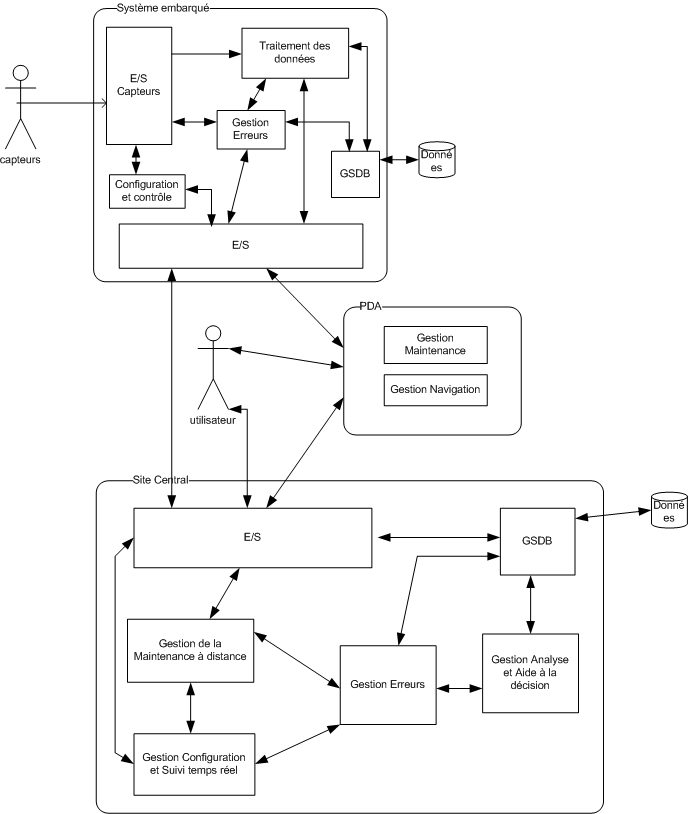
\includegraphics[width=11cm,height=12cm]{archiAppli.png}
\caption{Architecture Applicative du système}
\end{figure}

\subsection{Vérification du choix}
	Cette architecture applicative permet d'identifier les différents éléments et mécanismes du système à réaliser. Par souci de réutilisabilité et d’adaptabilité, le sous-projet doit être découpé en plusieurs ensembles successifs et complémentaires et sera développé de manière incrémentale. Cette démarche permet de développer des ensembles plus légers et en même temps.

\subsubsection{Système embarqué} Cette partie sert à gérer les activités du système embarqué, il en comprend

	\begin{itemize}
	    \item E/S capteurs : Il sert sert à l'acquisition les données en provenance des capteurs connectés et les transforme en valeur exploitable par le module Traitement. Il sert aussisert à traiter le signal électrique transmis par les capteurs.
	    \item Traitement des données :Il s'agit le coeur du système embarqué.  Il permet d'exploitation et de traitement des données à l’aide des microcontrôleurs intégrés. Il est chargé aussi le traitement des commandes reçues et d'opérations nécessaires à effectuer. Il gère aussi les capteurs et ainsi l'énergie.
	    \item GSDB : Gestion de la Base de données du système embarqué. 
	    \item Gestion des Erreurs : Détection et Diagnostics des dysfonctionnements dans le système.
	    \item Configuration : Sert à configurer le système (durée de période de transmise…) ainsi que les capteurs.
	    \item Communication: Gestion de la communication vers l’extérieur. Il réceptionne les commandes depuis le serveur et lui envoie les données acquises. 
	\end{itemize}

\subsubsection{Site central}

	\begin{itemize}
	    \item Analyse et Gestion Aide à la décision : elle est chargée d’analyser les statistiques, les données, les historiques. A partir de ces données, il peut générer les plannings optimaux pour les trajets de maintenance, les opérations à effectuer selon le cas. Egalement, il donnera le conseil sur la configuration du site et aussi des stations génériques.
 
	    \item Communication : Elle sert à la communication vers l’extérieur : envoie les commandes au système embarqué, réceptionne les informations, les demandes... 
	    \item GSDB : Gestion du stockage des données
	    \item Gestion des Erreurs : Détection et Diagnostics des dysfonctionnements dans le système.
	    \item Authentification d’utilisateur : sert à la vérification d’identité d’utilisateur afin d’autoriser l’accès aux ressources. Seules les personnes ayant les droit d’accès peuvent effectuer les opérations.
		\item Configuration et Commandes: responsable de la configuration et de traiter toutes sortes de commandes d’utilisateurs pour le site central ainsi que pour les systèmes embarqués. 

	\end{itemize}

\subsubsection{Système PDA}
	\begin{itemize}
	\item Gestion maintenance : Elle est chargée de la gestion de la maintenance à distance : reçoit les données envoyées par le site central et capable de modifier la maintenance/configuration d'un capteur précis. Il permettra aussi
de consulter le planning et les autres utiles informations.

	\item Gestion navigation : Il permettra aux caminoneurs de consulter leurs trajets, le planning, l'organisation d'une opération maintenance. Il permet aussi d'enovyer d demandes d'aide et d demandes de changement du trajet prévu. Il permet également d'envoyer les localisations des camioneurs

	\end{itemize}
